\def\tightlist{}
\documentclass[signature, dutch, biblatex]{deltares_report}
$if(highlighting-macros)$
$highlighting-macros$
$endif$
$if(csl-refs)$
% Pandoc citation processing
\newlength{\cslhangindent}
\setlength{\cslhangindent}{1.5em}
\newlength{\csllabelwidth}
\setlength{\csllabelwidth}{3em}
\newlength{\cslentryspacingunit} % times entry-spacing
\setlength{\cslentryspacingunit}{\parskip}
% for Pandoc 2.8 to 2.10.1
\newenvironment{cslreferences}%
  {$if(csl-hanging-indent)$\setlength{\parindent}{0pt}%
  \everypar{\setlength{\hangindent}{\cslhangindent}}\ignorespaces$endif$}%
  {\par}
% For Pandoc 2.11+
\newenvironment{CSLReferences}[2] % #1 hanging-ident, #2 entry spacing
 {% don't indent paragraphs
  \setlength{\parindent}{0pt}
  % turn on hanging indent if param 1 is 1
  \ifodd #1
  \let\oldpar\par
  \def\par{\hangindent=\cslhangindent\oldpar}
  \fi
  % set entry spacing
  \setlength{\parskip}{#2\cslentryspacingunit}
 }%
 {}
\usepackage{calc}
\newcommand{\CSLBlock}[1]{#1\hfill\break}
\newcommand{\CSLLeftMargin}[1]{\parbox[t]{\csllabelwidth}{#1}}
\newcommand{\CSLRightInline}[1]{\parbox[t]{\linewidth - \csllabelwidth}{#1}\break}
\newcommand{\CSLIndent}[1]{\hspace{\cslhangindent}#1}
\renewcommand{\FrontCover}{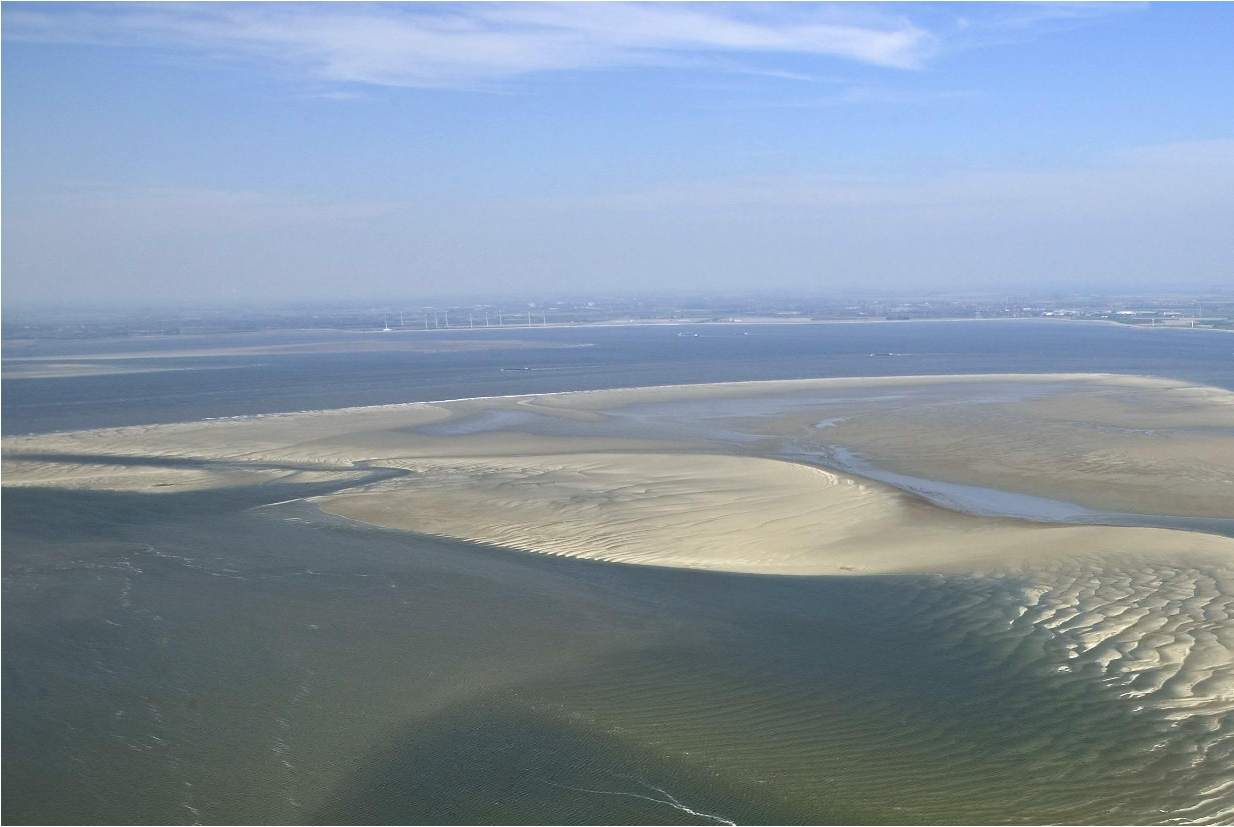
\includegraphics[width=182mm,height=182mm]
{Figuren/cover/getijdenland.pdf}}
\coverPhoto{}
$endif$
\begin{document}
\title{Eerstelijn Rapportage Westerschelde}
\subtitle{1998 - 2020}
\author{Deltares}
\partner{}

\client{Rijkswaterstaat WVL, VNSC}
\contact{Albert Mulder}
\reference{}
\keywords{hydrodynamiek, waterkwaliteit, zwevend stof, sediment, biota, fytoplankton}

\version{2021}
\date{16-08-2022}
\projectnumber{1209394}
\documentid{}
\status{definitief}
\disclaimer{}
% \references{References}

\authori{Willem Stolte, Bob van Rongen}
\organisationi{Deltares}
\versioni{1.0}
\datei{22-02-2023}
\revieweri{Peter Herman}
\approvali{Paul Saager}
\publisheri{Deltares}

\summary{
Deze rapportage bevat de beschikbare hydrodynamische, fysisch-chemische en biologische data (alleen fytoplankton) in de periode 1996 tot en met 2020 voor de Westerschelde en de monding. Het is een eerste weergave van de beschikbare data en beschrijft enkel ‘wat men in de meetresultaten ziet’. Het bevat een interpretatie van de gegevens op basis van een eenvoudige analyse. De rapportage is opgesteld in het kader van de OntwikkelingsSchets 2010 en vormt een van de bouwstenen voor de vergunningverlening van de derde verdieping van het Schelde-estuarium.
}
\deltarestitle
%------------------------------------------------------------------------------

% Text body

$body$

%------------------------------------------------------------------------------
\end{document}
